\documentclass[pdf]{beamer}
\mode<presentation>{}
\usepackage{minted}
\usepackage{tikz}
\usepackage{pgffor} %% gives looping with \foreach
\usepackage[absolute,overlay]{textpos}
\usepackage{lmodern} %% scalable latin characters
\usetikzlibrary{arrows,shapes,backgrounds}
\usepackage{multirow}
\usepackage{listings} %% another package for code related stuff
%\usepackage[fleqn]{amsmath}

%% stuff for minted
\definecolor{mintedBg}{rgb}{0.95, 0.95, 0.95}
\definecolor{blockBg}{rgb}{0.6, 0.6, 0.95}
\definecolor{rnaColor}{rgb}{0, 0.6, 0}
\definecolor{cdsColor}{rgb}{0, 0.4, 0.4}
\definecolor{rnaPol}{rgb}{0.8,0,0.8}
\definecolor{ribosomeCol}{rgb}{0.5,0.5,0.1}
\definecolor{protColor}{rgb}{0.6,0,0.6}
%% colours for nucleotides:
\definecolor{dACol}{rgb}{0.5, 0.5, 0}
\definecolor{dCCol}{rgb}{0.8, 0, 0}
\definecolor{dGCol}{rgb}{0, 0.8, 0}
\definecolor{dTCol}{rgb}{0, 0, 0.8}

\definecolor{navy}{rgb}{0, 0, 0.6}
\definecolor{pur}{rgb}{0, 0, 0.6}
\definecolor{pyr}{rgb}{0.6, 0, 0.2}

\definecolor{purple1}{rgb}{1.0, 0, 0.6}
\definecolor{purple2}{rgb}{0.8, 0, 0.8}
\definecolor{purple3}{rgb}{0.6, 0, 1.0}
%% define styles for different codes
\newminted{cpp}{linenos, bgcolor=blockBg, fontsize=\footnotesize}
%% then use \begin{cppcode}
\newminted{c}{linenos, bgcolor=mintedBg, fontsize=\footnotesize}
\newminted{perl}{linenos, bgcolor=mintedBg, fontsize=\footnotesize}
\newminted{r}{linenos, bgcolor=mintedBg, fontsize=\footnotesize}

%% a command to define a subheading
\newcommand\subHeading[1]{
  \par\bigskip {\Large\bfseries#1}\par\smallskip
}

%% I detest indentation in footnotes etc, so try this:
\makeatletter
\renewcommand\@makefntext[1]{\noindent\makebox[0em][r]{\@makefnmark}\tiny#1}
\makeatother
%% the makeatletter and makeatother are required to allow me to
%% to change the macro beginning with an @. (though when I call it
%% I don't use the @ ... 

\setlength\parskip{0.5em}
\setlength\parindent{0ex}

%% to have footnotes without references. This from tex.stackexchange.com
\newcommand\blfootnote[1]{%
  \begingroup  %% this makes it a local redefinition
  \renewcommand\thefootnote{}\footnote{#1}%
  \addtocounter{footnote}{-1}  % this adjusts the footnote counter
  \endgroup
}


%% to draw a pair of genes..
\newcommand{\genePair}[3][]{
        \draw [-,#1] (#2-1,#3) -- (#2+1,#3);
        \draw [-,line width=2, purple1] (#2-0.5,#3) -- (#2+0.5,#3);
        \draw [-,#1] (#2-1,#3-0.5) -- (#2+1,#3-0.5);
        \draw [-,line width=2, purple3] (#2-0.5,#3-0.5) -- (#2+0.5,#3-0.5);  
}

\title{Looking at numbers}
\subtitle{Summarising number collections}
\author{Martin Jakt}

\begin{document}

\begin{frame}
\titlepage
\end{frame}

\begin{frame}{Summarising what?}
  \begin{itemize}
  \item Values
  \item Variances
  \item Differences
  \end{itemize}

  Usually for a data set we wish to make some conclusion. That is to
  summarise the numbers to a single value. Today we will start to look
  at how we do this.
\end{frame}

\begin{frame}{Value summaries}

{
\bfseries{Average?}
}

\begin{description}
\item[Mean] \pause Sum divided by number of values
\item[Median] \pause Center of distribution
\item[Mode] \pause Most common value
\end{description}

\pause
The typical mean value is known as the \textcolor{blue}{\emph{arithmetic}} mean,
but we also have the \textcolor{blue}{\emph{geometric}} mean and median values,
as well as the \textcolor{blue}{\emph{harmonic}} mean.

\end{frame}

\begin{frame}{Value summaries (2)}
  if X is the set of numbers (3, 4, 5, 5, 6, 6, 6, 6, 7):

  \small
  \begin{description}
  \item[Mean] 
    $ mean(X) = \frac{3 + 4 + 5 + 5 + 6 + 6 + 6 + 6 + 7}{9} = \frac{48}{9} = 5.3 $
  \item[Median] If X is ordered and n is the number of members\\
    $ median(X) = X_{n/2} = X_{4.5} = \frac{X_4 + X_5}{2} = 5.5 $
  \item[Mode] The most common number. May be undefined\\
    $ mode(X) = 6 $
  \end{description}
\end{frame}

\begin{frame}{Variability summaries}

for a set of values of size n.

\begin{description} \pause
\item[range] max - min (signed or unsigned) \pause
\item[variance] sum of squared deviates (difference between values and the
  group mean) divided by n or (n-1) .\pause
\item[standard deviation] square root of the variance. \pause
\item[standard error] standard deviation of the summary statistic (usually
  mean). Equal to the standard deviation divided by the square root of n. \pause
\item[MAD] Median Absolute Deviation. The median of absolute deviations around
  the median.
\end{description}
\end{frame}

\begin{frame}{variance, standard deviation, standard error (1)}
  \small
  For a set of $n$ values $x$
  which has a mean value of $\overline{x}$
  we estimate the variance of the population from which $x$ has been
  sampled ($X$) as:
  
  $$ X_v \sim \frac{\sum_{i=1}^{n}{(x_i - \overline{x})^2}}{n-1} $$ 
  
  Here, $\overline{x}$ and $X_v$ are estimates of the 
  mean and variance of the population from which $X$ has
  been sampled.

  If we know all of the values in $X$ we directly calculate the variance as:
  $$X_v = \frac{\sum_{i=1}^{N}{(X_i - \overline{X})^2}}{N} $$ 

  Where $N$ is the number of values in $X$. The standard deviation, $X_{sd}$
  is simply the square root of the variance. It is often represented by the
  greek letter $\sigma$:
  $$\sigma = X_{sd} = \sqrt{X_v}$$ 

\end{frame}

\begin{frame}{variance, standard deviation, standard error (2)}
  The standard deviation ($X_{sd}$) is an estimate of how much values of
  $X$ vary (\textcolor{blue}{the population standard deviation}). 

  The \textcolor{blue}{standard error of the mean} ($x_{se}$) 
  is a measure of the variability of an estimate of
  the mean of $X$ based upon $n$ samples (i.e. $\overline{x}$). It is:
  $$ x_{se} = \frac{X_{sd}}{\sqrt{n}} $$

  $x_{se}$ corresponds to the standard deviation of a set of mean values
  obtained by repeatedly sampling $n$ values from the population $X$.
\end{frame}

\begin{frame}{mean, standard deviation, standard error}
  \vspace{-1cm}
  \begin{figure}
    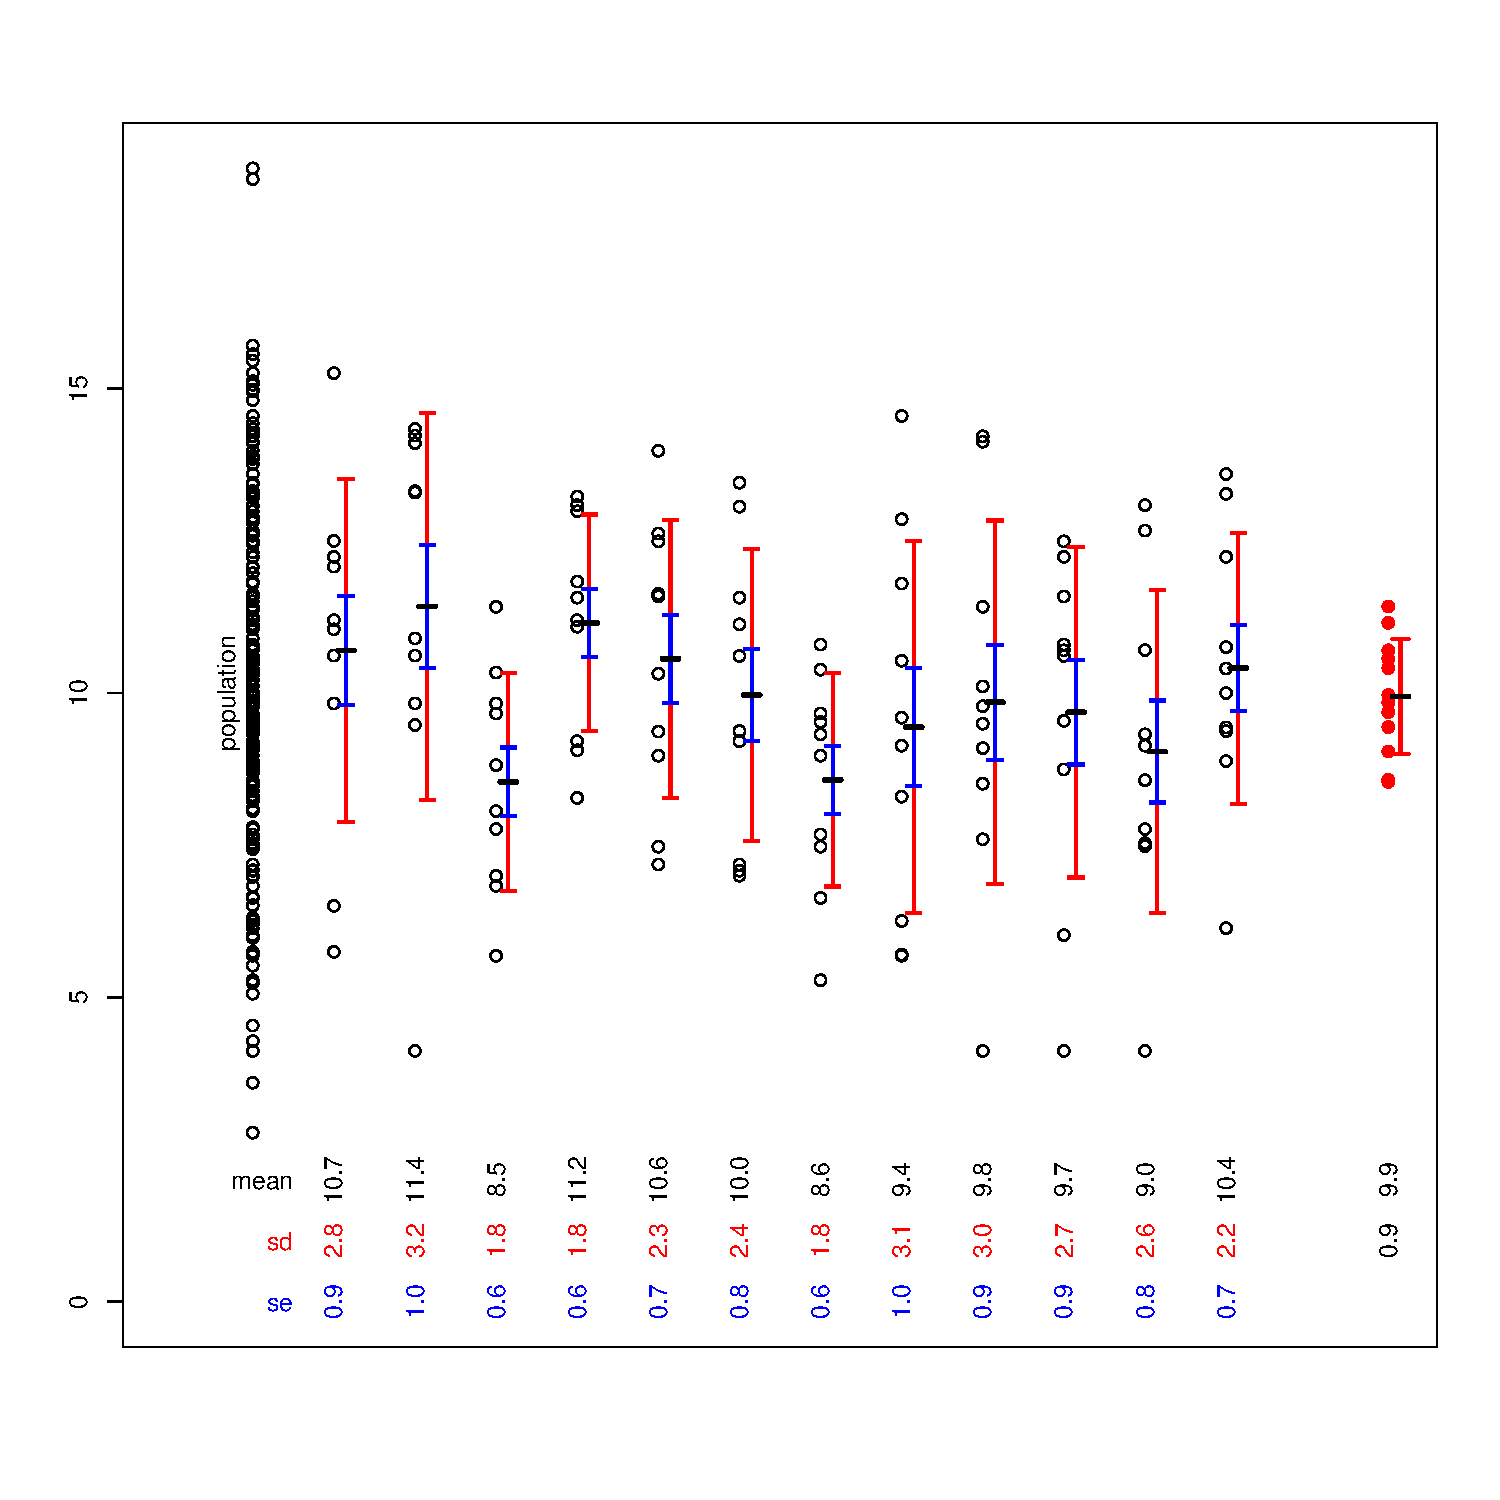
\includegraphics[width=0.7\textwidth]{R/mean_sd_se}
  \end{figure}
  \vspace{-1cm}
  \footnotesize 12 sets of 10 values were sampled from 200 normally
  distributed values and mean, standard deviation and standard error
  calculated. The standard errors of the sampled sets approximate the standard
  deviation of the mean values (right-most column).
\end{frame}

\begin{frame}{Difference summaries}

For two sets of values X and Y, these provide a summary of the difference
between X and Y.

\begin{itemize}
\item \textcolor{blue}{Difference of a summary measure}\\ eg. mean(X) - mean(Y)
\item \textcolor{blue}{Difference normalised by variance}\\ eg. (mean(X) -
  mean(Y)) / var(X,Y).
\item \textcolor{blue}{Seperation of values}\\ eg. if(X \textgreater Y) min(X) - max(Y)
\item \textcolor{blue}{Pairwise differences}\\ the average difference of
  paired values or all against all differences.
\item \textcolor{blue}{...} anything that suits the question asked.
\end{itemize}

\end{frame}

\begin{frame}{Sampling from random numbers}
  \begin{itemize}
  \item  Most statistical measurements are based on an idea of random sampling from
    populations of some specified distribution.
  \item We can easily simulate this and hence, check whether our use of an equation
    makes sense.
  \item This allows us to approach statistics in an experimental rather
    than rigidly mathematical manner.
  \item R to the rescue!
  \end{itemize}
\end{frame}

\begin{frame}[fragile]{Averages from random numbers (1)}

Easy in R:
\begin{rcode}
  n <- 100 ## the number of averages
  k <- 10  ## the size of each set of numbers
  ## something to store the numbers in
  m <- vector(mode='numeric', length=n) 
  ## the range from which we sample 
  minV <- 0
  maxV <- 10 
  ## loop to obtain mean values
  for(i in 1:n){
    m[i] <- mean( sample(minV:maxV, k, replace=TRUE) )
  }
  plot(m)
\end{rcode}

provides means of sets of k numbers randomly sampled from the range minV to maxV.

\end{frame}

\begin{frame}{Averages from random numbers (1)}

\begin{figure}[ht]
  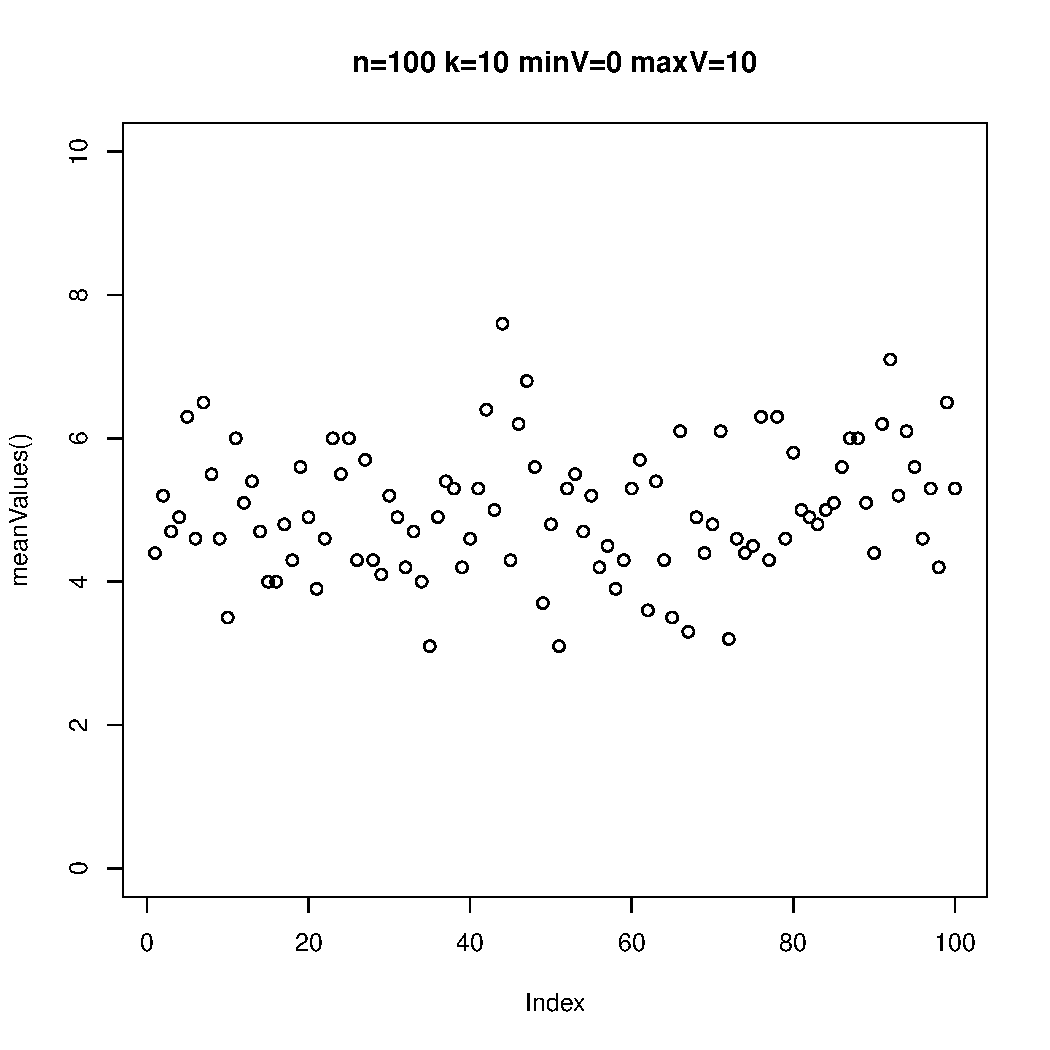
\includegraphics[width=0.8\textwidth]{images/averages1}
\end{figure}
\end{frame}

\begin{frame}{More averages}

\begin{figure}[ht]
  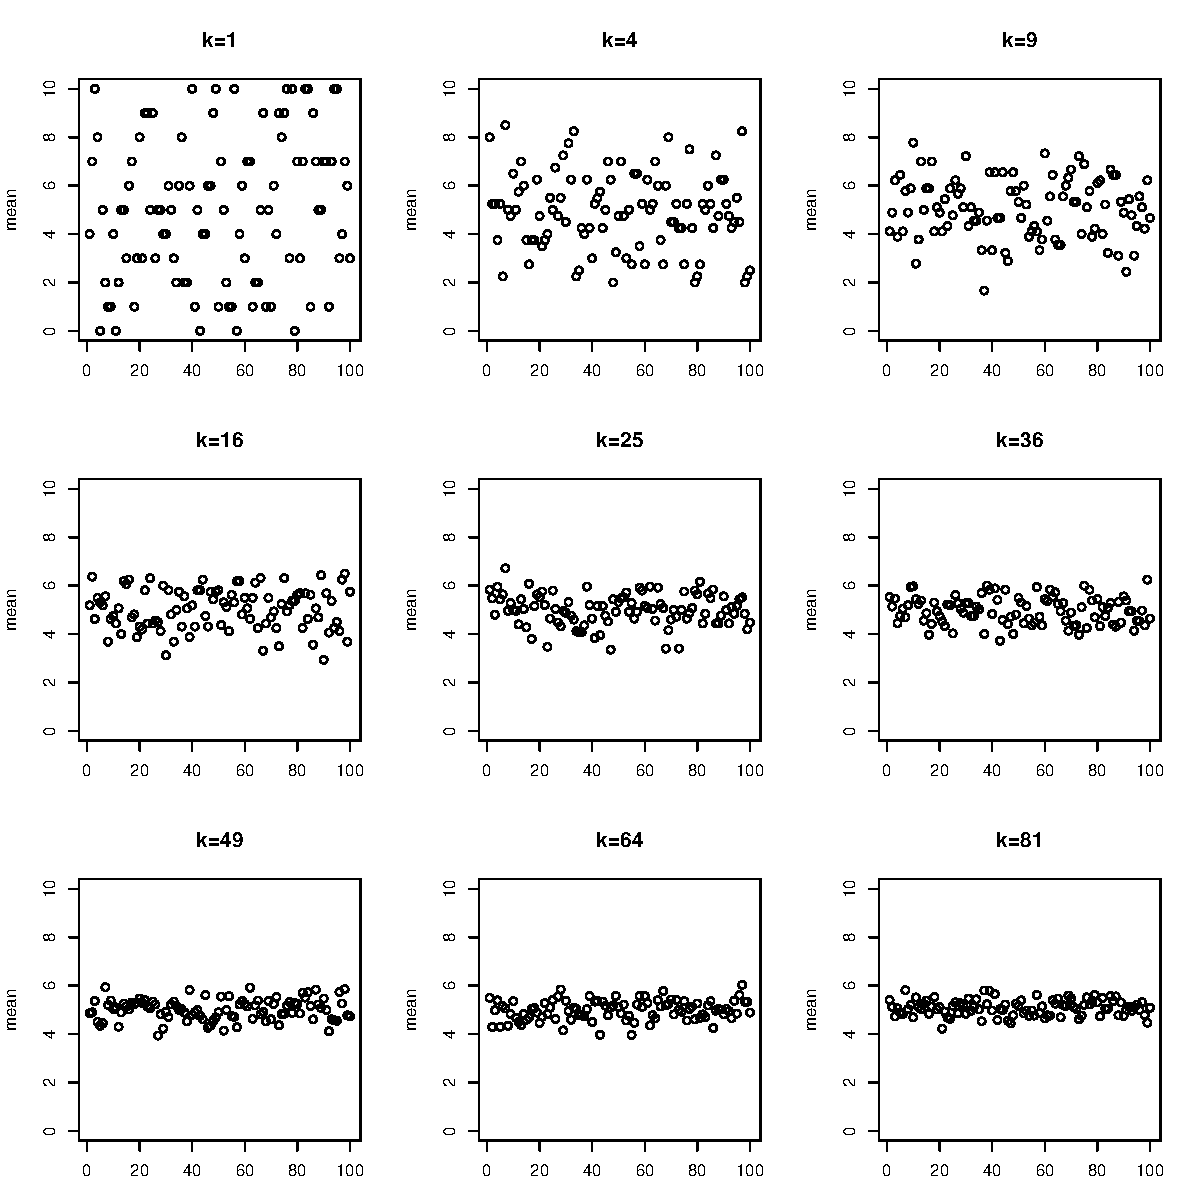
\includegraphics[width=0.7\textwidth]{images/averages2}
\end{figure}
\small  n=100 minV=0 maxV=10
\end{frame}

%% \begin{frame}{Medians}
%% \begin{figure}[ht]
%%   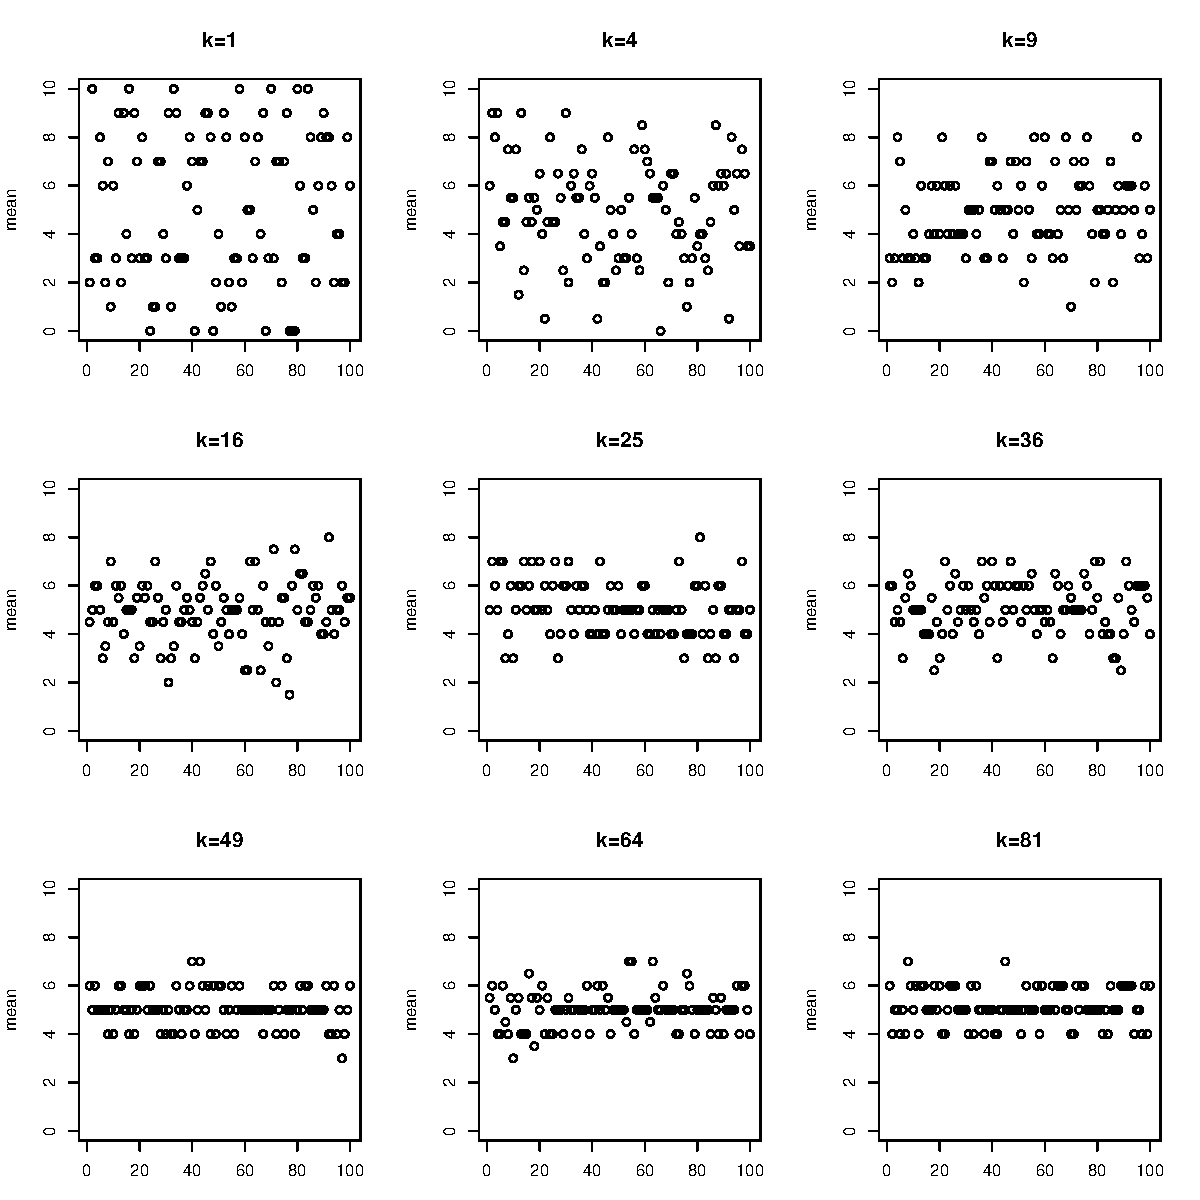
\includegraphics[width=0.7\textwidth]{images/medians1}
%% \end{figure}
%% \end{frame}

\begin{frame}[fragile]{Distributions}

\begin{rcode}
    meanValues <- function( n=100, k=10, minV=0, maxV=10 ){
      m <- vector(mode='numeric', length=n)
      for(i in 1:n){
        m[i] <- mean( runif(k, min=minV, max=maxV) )
      }
      m
    }

    m <- meanValues( n=10000, k=10, minV=0, maxV=10 ) 
    mh <- hist( m, breaks=seq(0, 10, by=0.25))
    m.norm <- dnorm( mh$mids, mean=mean(m), sd=sd(m) )
    m.bp <- barplot( mh$density/sum(mh$density),
                     main=paste('mean=', 
                     sprintf('%.2f', mean(m)),
                     ' standard deviation=', 
                     sprintf('%.2f', sd(m)), sep=''),
                     ylim=c(0,0.12))
    lines(m.bp, m.norm/sum(m.norm), type='b', col='red')
    ## in R $ is used to access members of named lists
    ## don't confuse it with how it's used in Perl
\end{rcode}
\end{frame}

\begin{frame}{runif?}
  What's this \textcolor{blue}{runif} thing?

  R has a number of functions that provide random sampling from
  different distributions. The simplest of these is the \textcolor{blue}{uniform}
  distribution (random numbers within a specified range). The \textcolor{blue}{r}
  stands for random. There are also related functions starting with
  \textcolor{blue}{d} and \textcolor{blue}{p} that can be used to obtain
  distributions and the probability of observing specific values within a specified
  distribution.

  When you use R to do a t-test, the p-value is obtained from the \textcolor{blue}{pt}
  function. Other tests generate values with different distributions and
  these will use the corresponding functions.
\end{frame}

\begin{frame}{dnorm?}
  and what about that \textcolor{blue}{dnorm} thing?

  \textcolor{blue}{dnorm} provides density values for the
  \textcolor{blue}{normal} distribution. 

  It's part of the same family of functions as \textcolor{blue}{runif}
  and \textcolor{blue}{dunif}. We can use it to compare the distribution
  of our mean values to a theoretical normal distribution.
\end{frame}

\begin{frame}{A pretty normal distribution}
  \begin{figure}[ht]
    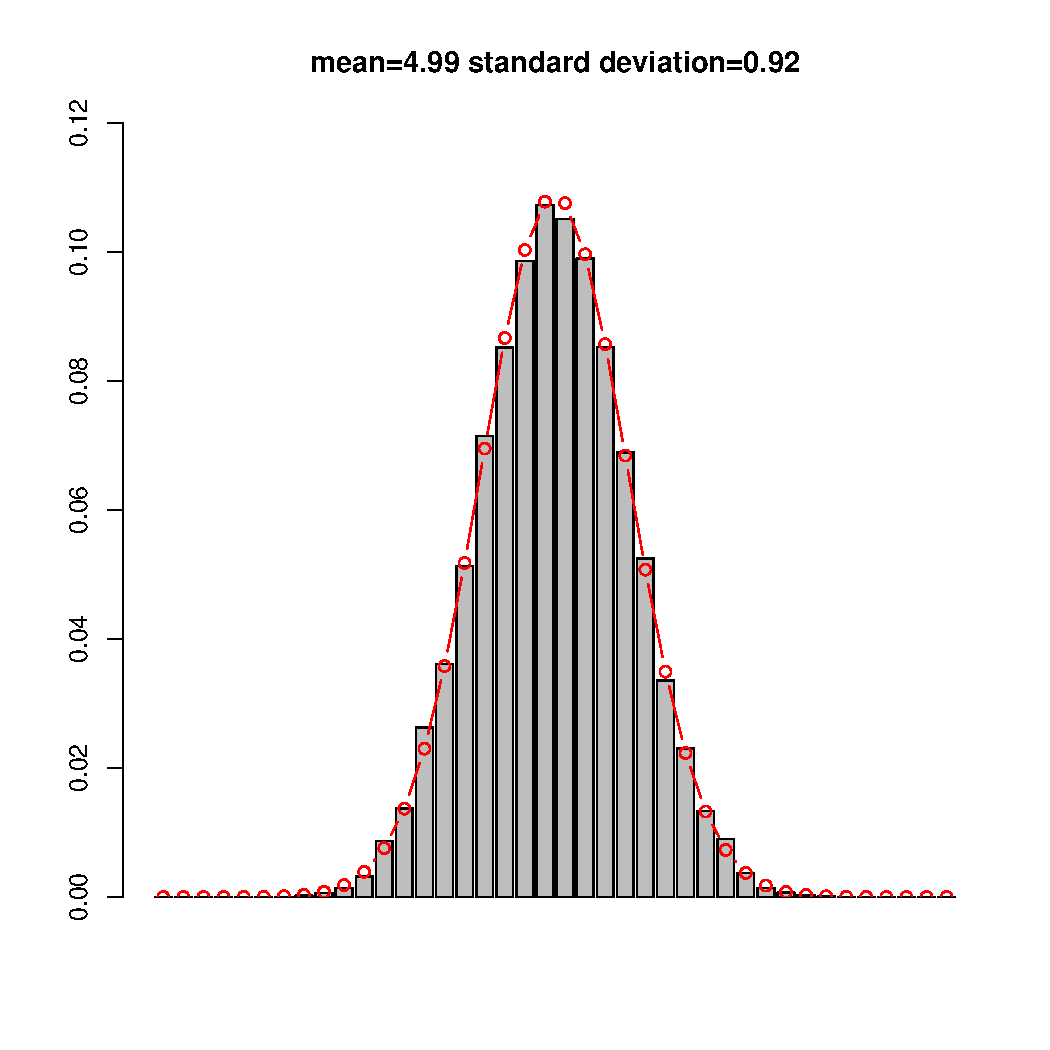
\includegraphics[width=0.7\textwidth]{images/dist2}
  \end{figure}
\end{frame}

\begin{frame}{More normal distributions}
  \begin{figure}[ht]
    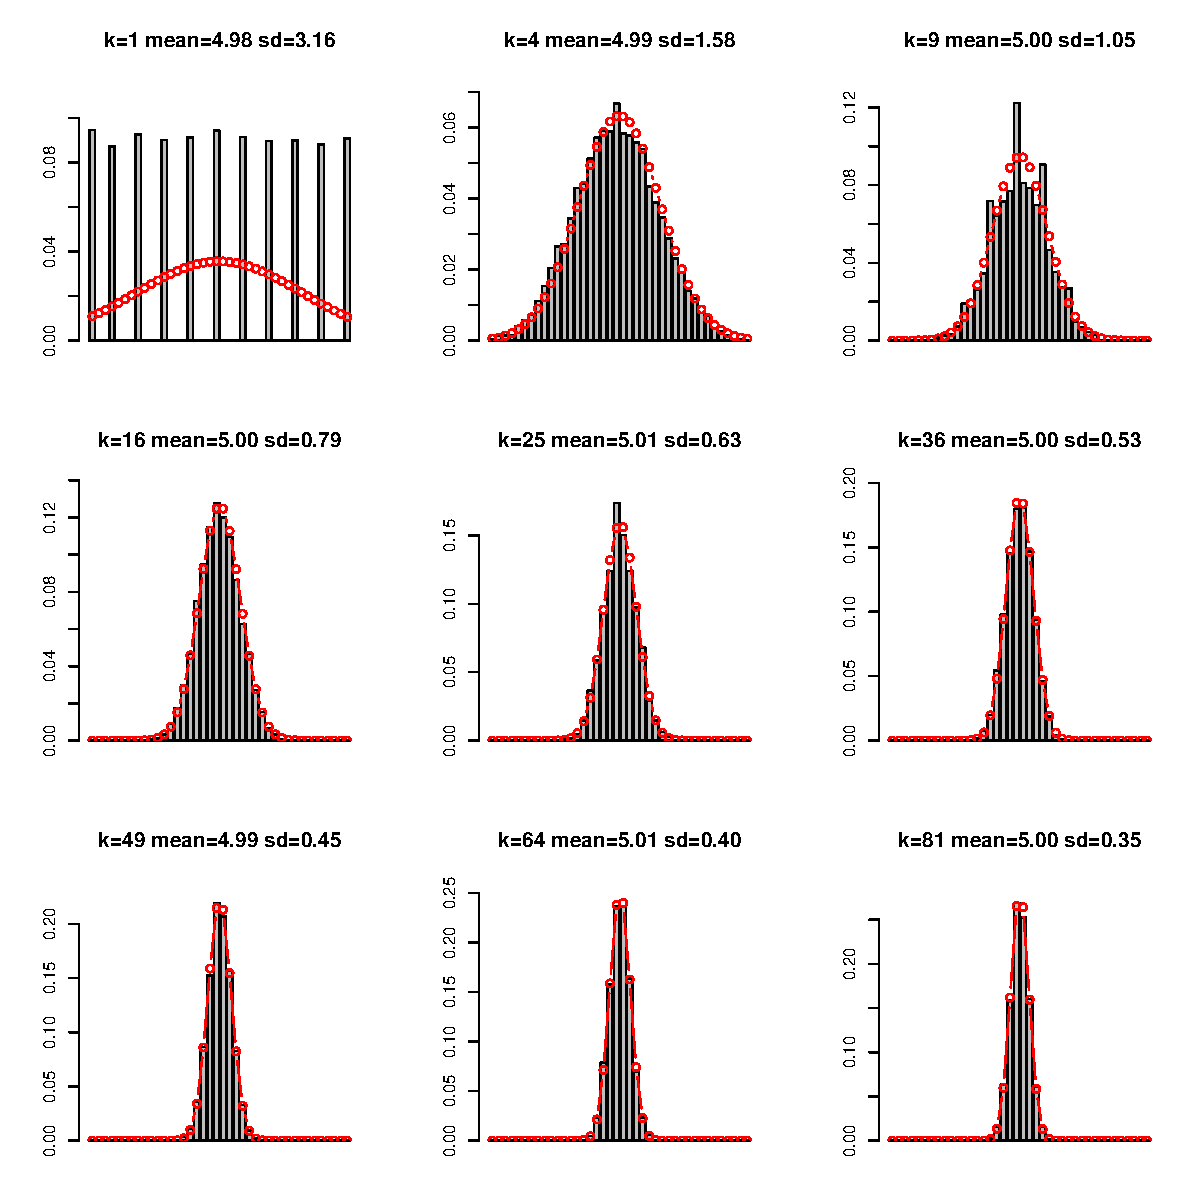
\includegraphics[width=0.7\textwidth]{images/dist3}
  \end{figure}

\end{frame}

\begin{frame}{The normal distribution}
\begin{itemize}
\item The most commonly used distribution\footnote{More like assumed, rather than used}
\item Required for common parametric statistical tests
\item Is generally true when the effect of unknown factors are added together
  (i.e. combined linearly).
\item For normal distributions, the mean, median and mode averages have the
  same value.
\end{itemize}

\footnotesize
Replicate (often) values assumed to vary due to the sum of a set of unknown
replicates $\Rightarrow$ normal distribution.
\end{frame}

\begin{frame}{The log normal distribution}
  If experimental measurements result from the product of random variables we
  obtain a normal distribution of log transformed values:

  $$
  log(x_1) + log(x_2) + log(x_3) = log( x_1 \times x_2 \times x_3 )
  $$
  
  This is often true in biological systems, and is the reason we frequently log
  transform values.

\end{frame}

\begin{frame}[fragile]{More stuff on the Normal distribution}
  \begin{rcode}
    m <- meanValues(n=10000, k=10, minV=0, maxV=10)
    m.sd <- sd(m)
    m.m <- mean(m)
    ## the number of values within 1, 2 and 3 
    ## standard deviations of the mean
    m.sd1 <- sum( abs(m - m.m) <= m.sd )
    m.sd2 <- sum( abs(m - m.m) <= 2 * m.sd)
    m.sd3 <- sum( abs(m - m.m) <= 3 * m.sd)
  \end{rcode}

  m.sd1 : 6790\\
  m.sd2 : 9534\\
  m.sd3 : 9984

  i.e. 67\% and 95\% of values lie within one and two standard deviations of
  the mean respectively.

  This is true for all normal distributions regardless of mean and standard
  deviation.
\end{frame}

\begin{frame}{More stuff visualised}
  \begin{figure}[ht]
    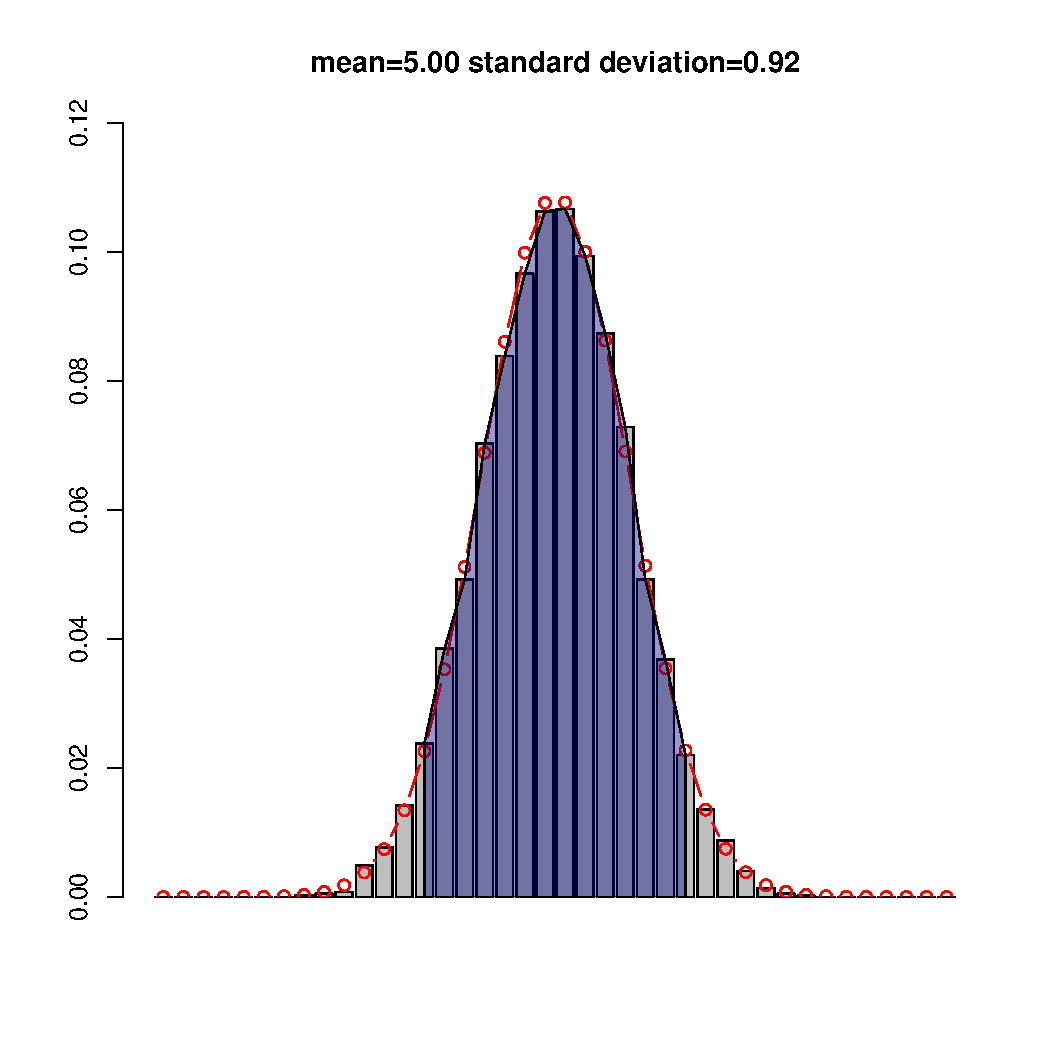
\includegraphics[width=0.7\textwidth]{images/dist4}
  \end{figure}
  \vspace{-8ex}
  The area within 2 standard deviations holds about 95\% of the values.
\end{frame}

\begin{frame}{Experimental data}
  \begin{itemize}
  \item Given a simple experiment, where some parameter, $p$ has been measured in
    control ($p_{ctl}$) and treatment ($p_{trt}$) subjects, we (often) assume that the
    values of $p$ can be
    considered as random samples from two normal distributions
    $d_{ctl}$ and $d_{trt}$.
  \item The number of replicates from each sample is equivalent to the number
    of samples obtained from each underlying distribution.
  \item The null hypothesis is that $p_{ctl}$ and $p_{trt}$ have been sampled
    from identical distributions.
  \item The alternative hypothesis is that they have been sampled from different
    distributions.
  \end{itemize}
  
  Statistical tests attempt to estimate the probability that the null
  hypothesis is true.
\end{frame}


\begin{frame}[fragile]{Exploring the probabilites of differences in mean values}
  Create 1000 sets of pairs of values sampled from the same (normal)
  distribution. That is where the \textcolor{navy}{null hypothesis} is true:
  \begin{rcode}
    ## use a mean of 0, and a standard deviation of 1
    n <- 10000
    sd <- 1
    m <- 0
    ## k is equivalent to the number of replicates 
    ## for each sample class in an experiment
    k <- 10
    ## two vectors for storing the means in
    X <- vector(mode='numeric', length=n)
    Y <- vector(mode='numeric', length=n)
    for(i in 1:n){
      X[i] <- mean( rnorm(k, mean=m, sd=sd) )
      Y[i] <- mean( rnorm(k, mean=m, sd=sd) )
    }
    ## look at the distribution of the differences:
    plot(X - Y)
    h <- hist( X - Y, breaks=40 )
  \end{rcode}

\end{frame}

\begin{frame}{Differences of means}
\begin{figure}[ht]
  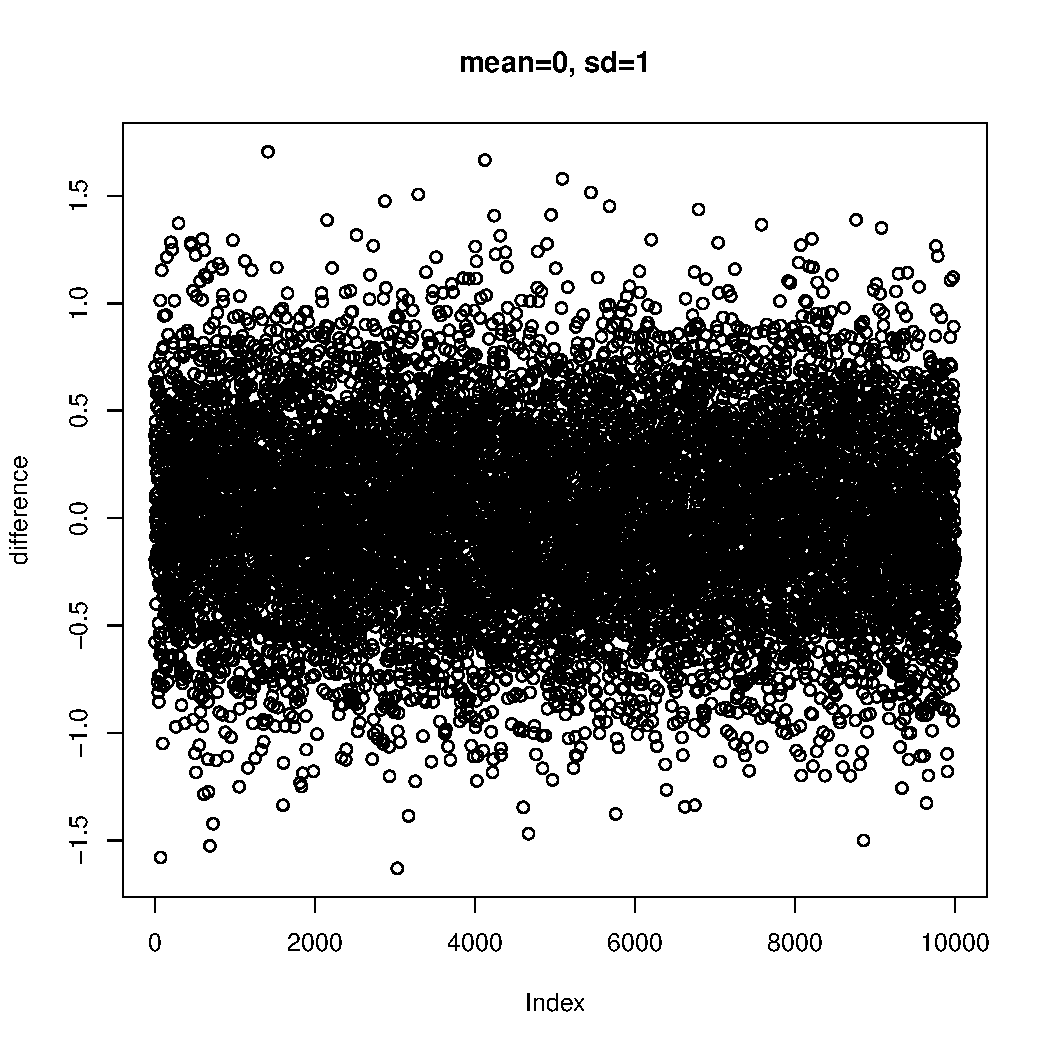
\includegraphics[width=0.7\textwidth]{images/differences1}
\end{figure}
\end{frame}

\begin{frame}{Distribution of differences}
\begin{figure}[ht]
  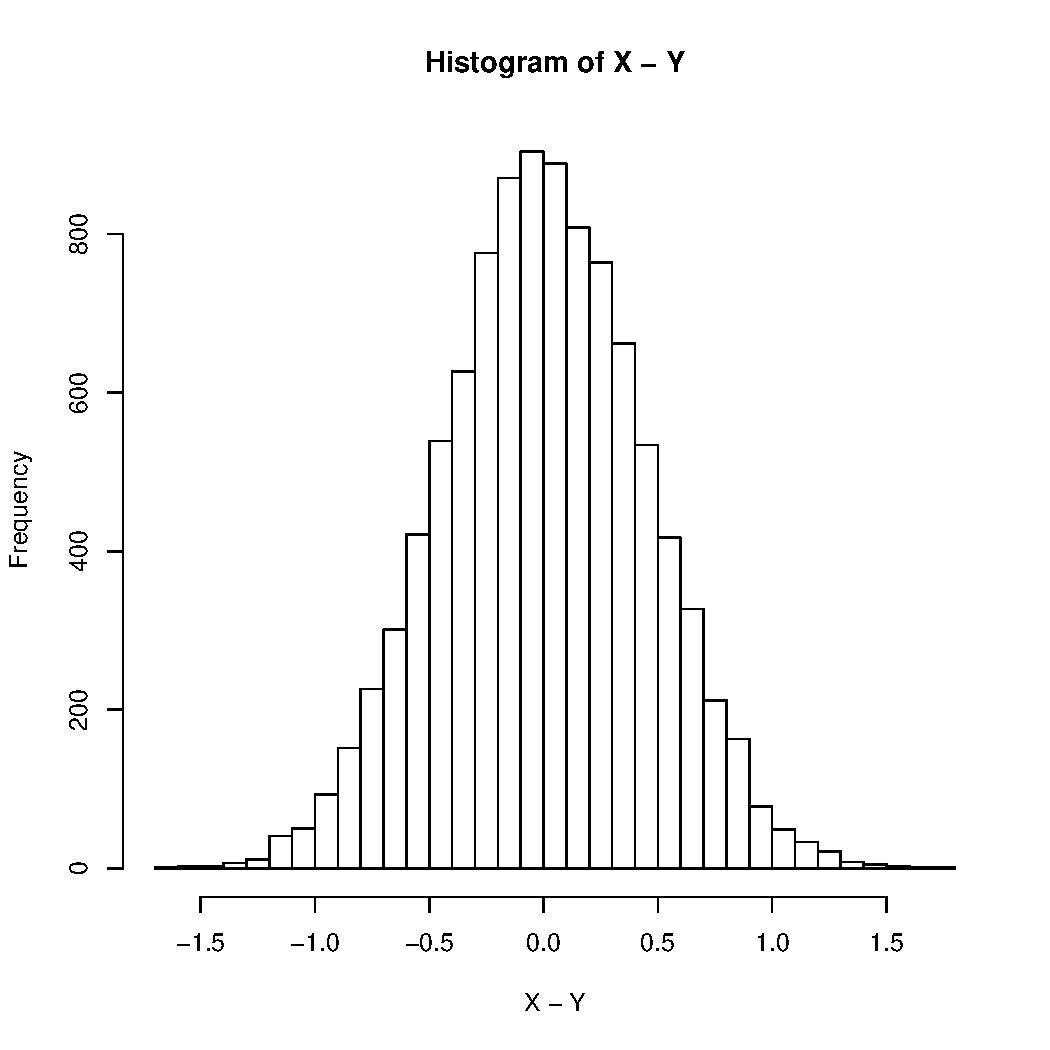
\includegraphics[width=0.65\textwidth]{images/diffDist}
\end{figure}
\vspace{-4ex}
\footnotesize
Normal distribution with mean=0 and standard deviation of 0.44.\\
Hence $\sim$0.05 chance of having an absolute difference of more than 0.88. 
\end{frame}

\begin{frame}{Experiment simulation}
  In the previous slides we simulated 10,000 experiments comparing two
  different conditions where we had 10 replicates from each sample, and where
  the null hypothesis was true.

  Under the assumptions given (normal distributions with an equal variance of the X and Y
  variables) we can use this distribution to test the null hypothesis. For
  a given experiment we have only a 5\% chance of seeing an absolute
  difference larger than 0.88.

  Normally we don't know so much about what the numbers should be so, we need
  to estimate these from the experimental data.
\end{frame}

\begin{frame}{the t-test}
  The t-statistic $t$ for the difference between the means of $X$ and $Y$
  is :

  $$
  \frac{\overline{X} - \overline{Y}}{sd(X,Y)}
  $$
  
  where $sd(X,Y)$ is a measure of the overall variance of the measurement. 
  If sample sizes and variances can be assumed to be equal:

  $$
  t = \frac{\overline{X} - \overline{Y}}{ \sqrt{(s^2_{X} +
      s^2_{Y})}\cdot\sqrt{\frac{1}{n}}}
  $$
  
  Where $s^2_X$ and $s^2_Y$ are the squared standard deviations of X and Y
  (this is the same as their variances).
  
\end{frame}

\begin{frame}{t to p}
  To get a probability (p-value) of the null hypothesis being true, we can again
  simply do some random sampling to see what the distributions of $t$ are for
  a given variance under the null hypothesis. Given a standard deviation of 4
  for both X and Y and 10 replicates each we would get:
  
  $$
  t = \frac{\overline{X} - \overline{Y}}{\sqrt{4^2 +
      4^2}\cdot\sqrt{\frac{1}{10}}}
  $$

  Again, we can simply simulate these numbers:

\end{frame}

\begin{frame}[fragile]{t to p in R}
  \begin{rcode}
    N <- 10000 ## the number of samples of t
    k <- 10    ## number of replicates (n) for each group
    s <- 4     ## the standard deviation of the distributions
    t <- vector(mode='numeric', length=N)
    for(i in 1:N){
      X <- rnorm(n=k, mean=0, sd=s)
      Y <- rnorm(n=k, mean=0, sd=s)
      x.v <- var(X)
      y.v <- var(Y)
      x.m <- mean(X)
      y.m <- mean(Y)
      t[i] <- (x.m - y.m) / (sqrt(x.v + y.v) * sqrt(1/k))
    }
    h <- hist(t)
  \end{rcode}
\end{frame}

\begin{frame}{t to p: the distribution}
  \begin{figure}[ht]
    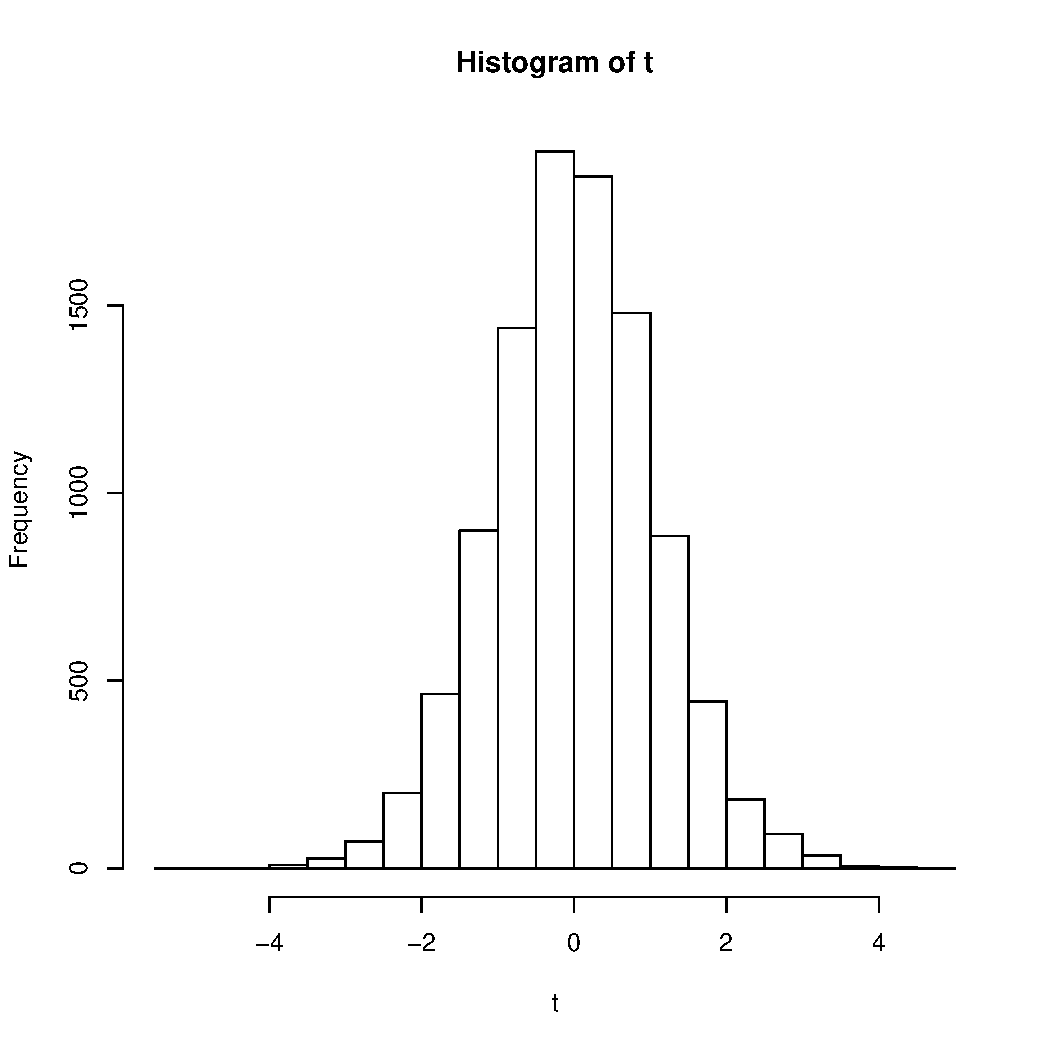
\includegraphics[width=0.7\textwidth]{images/tdist1}
  \end{figure}
\end{frame}

\begin{frame}[fragile]{for t already available}
  \small
  In R, you can directly get the distribution of t for a given number of
  degrees of freedom.

  Allowing us to check our experimental distribution:

  \begin{rcode}
    plot(h$mids, h$density, type='b', col='black')
    points(h$mids, dt(h$mids, df=(2*k-2)), type='b', col='red')
  \end{rcode}
  \begin{figure}[ht]
    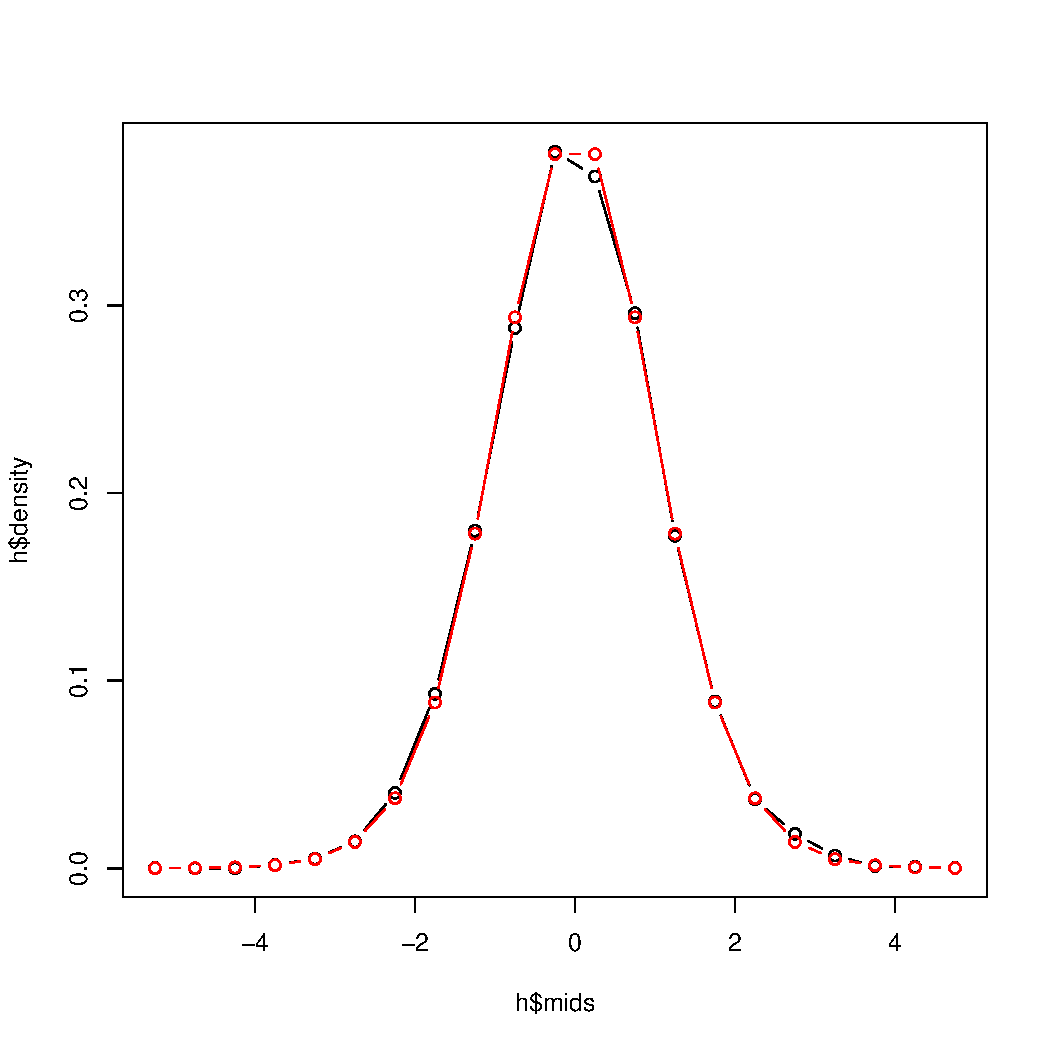
\includegraphics[width=0.5\textwidth]{images/tdist2}
  \end{figure}
\end{frame}

\begin{frame}[fragile]{the p-value}
  To get the p-value we can either check how many of the randomly
  generated values have a t-value greater or lower than the experimentally
  observed one. Eg. if we are interested in X \textgreater Y (positive
  p-values) we can do:
  \begin{rcode}
    ## to check the probability of observing a t-value 
    ## larger than a we can do:
    sum(t > a) / length(t)
    ## where t is the vector of t-values obtained
    ## when the null hypothesis is true
  \end{rcode}

  We can also use the built in function \texttt{pt}:
  \begin{rcode}
    pt(t, k*2-2)
    ## where k is the number of replicates (samples) 
    ## for each group
    ## k*2-2 is the number of degrees of freedom for the test.
  \end{rcode}
\end{frame}


\begin{frame}[fragile]{delta, t, p distributions}
  Mean of both distributions is 0, sd = 4 and replicate no=10 for both:
  \begin{figure}[ht]
    \begin{tikzpicture}[scale=0.5]
      \node [below right] at (0,10) {
        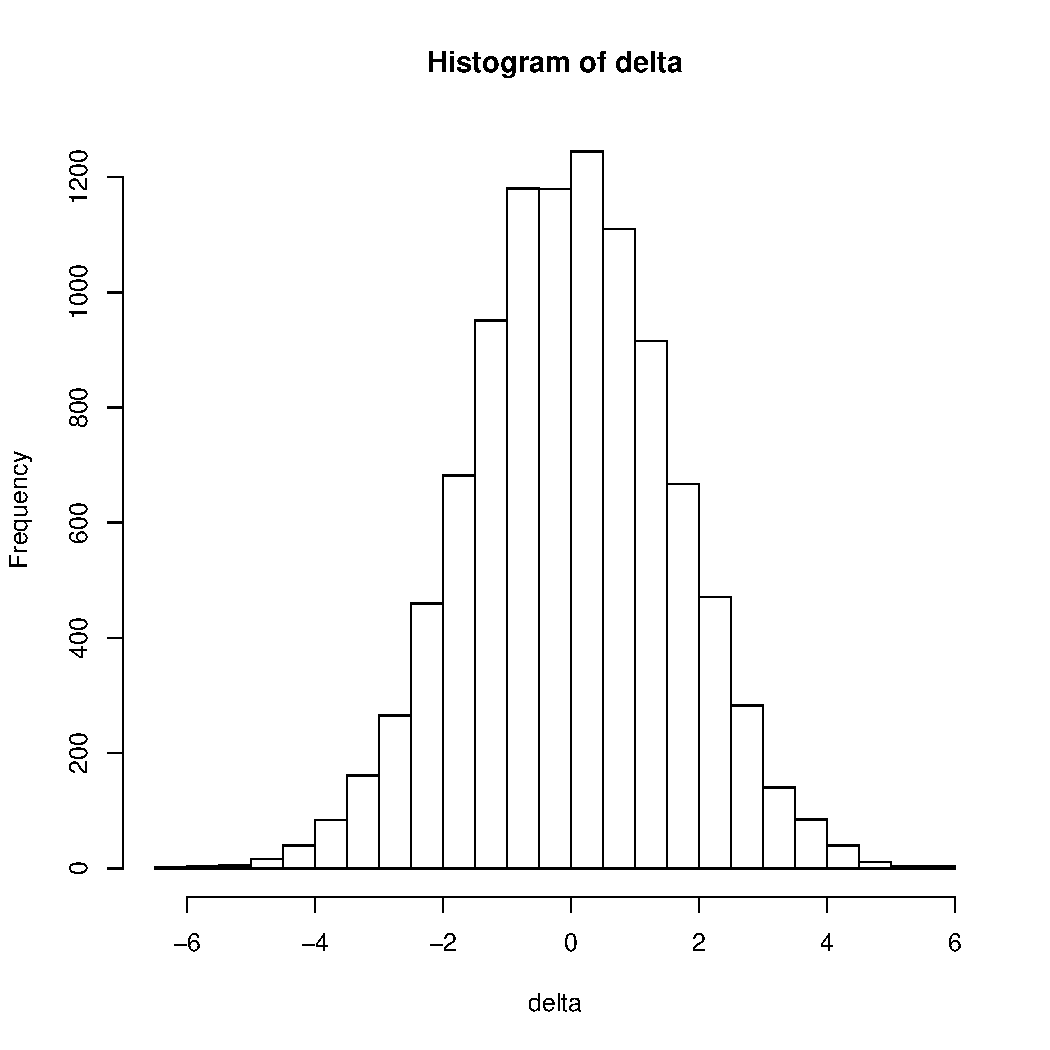
\includegraphics[width=.33\textwidth]{R/mean_diffs}};
      \pause
      \node [below right] at (8,10) {
        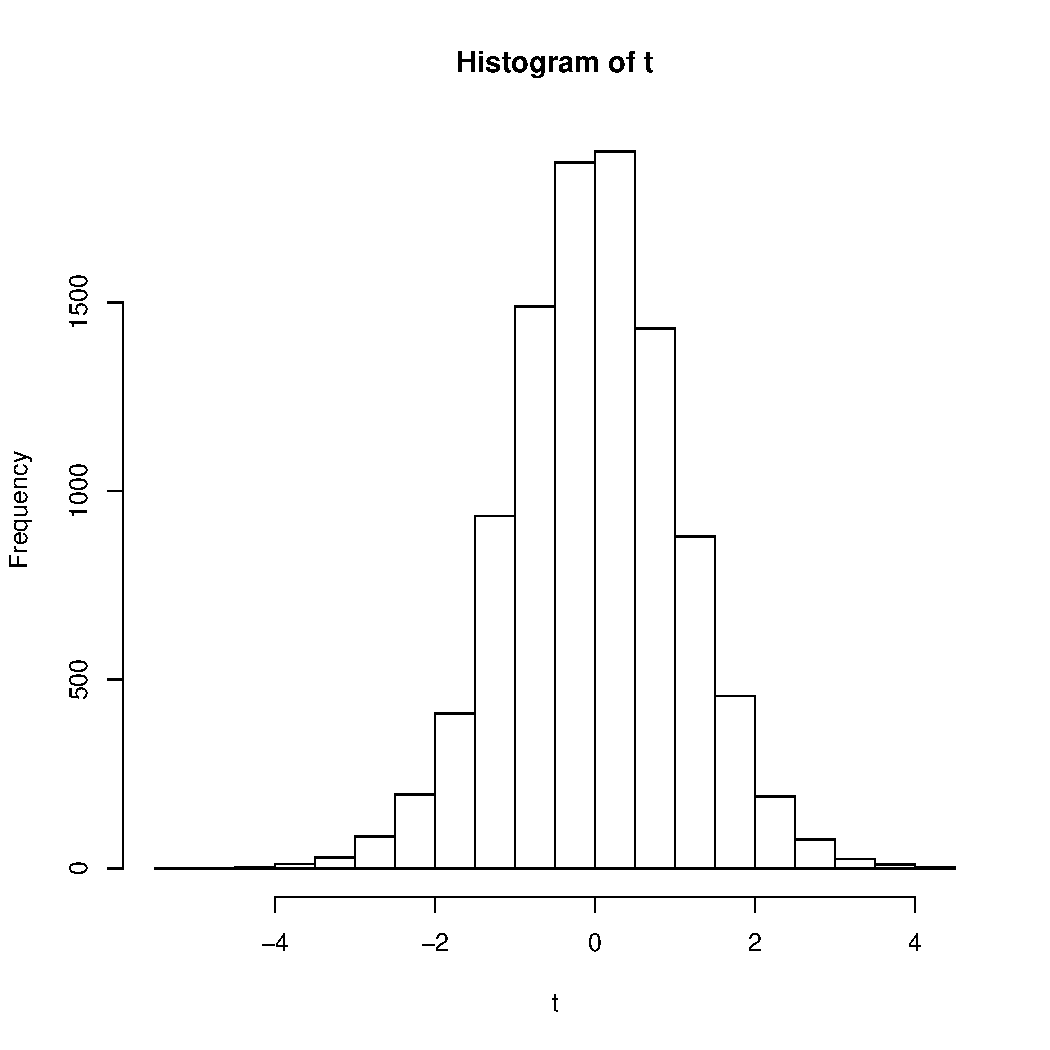
\includegraphics[width=.33\textwidth]{R/t_values}};
      \pause
      \node [below right] at (16,10) { 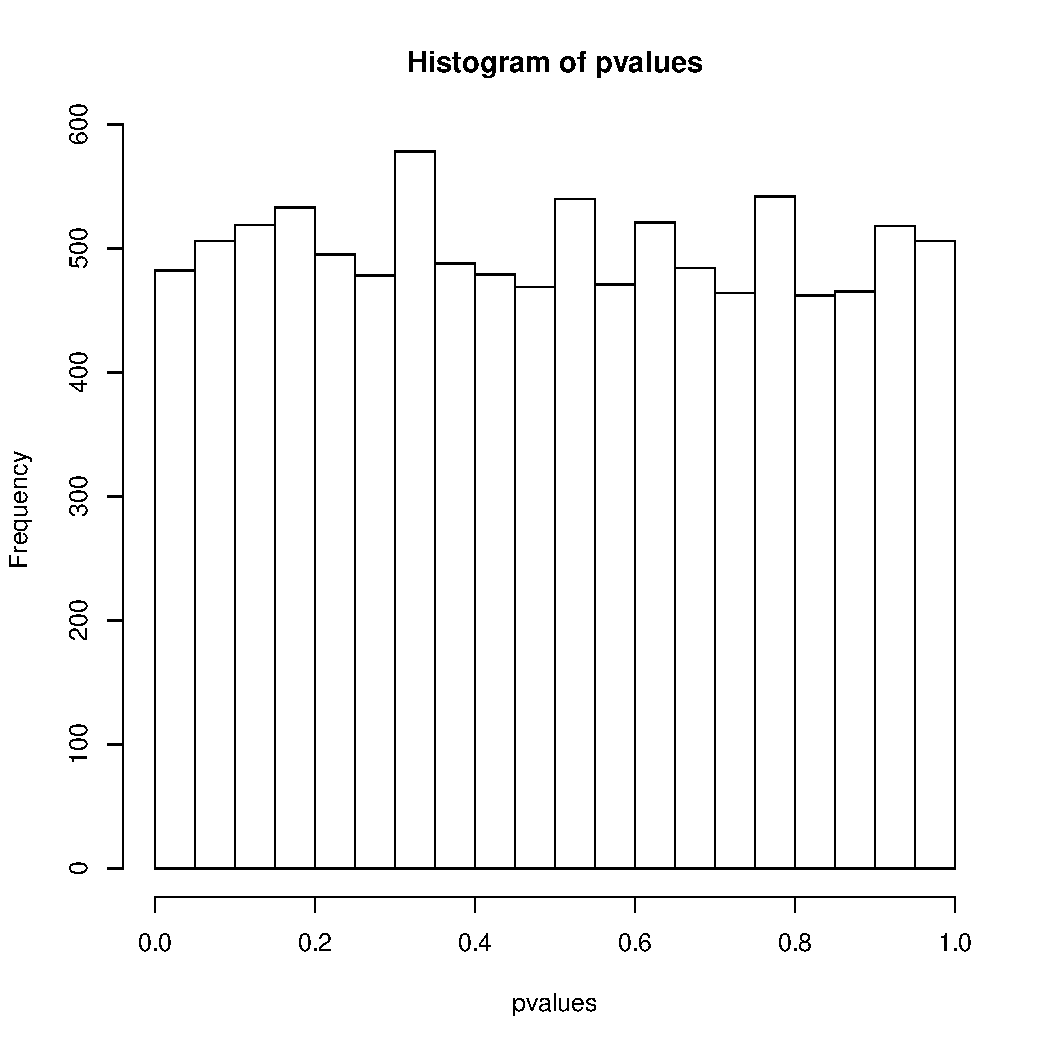
\includegraphics[width=.33\textwidth]{R/p_values}};
    \end{tikzpicture}
  \end{figure}
\end{frame}

\begin{frame}{under the \emph{null} hypothesis \emph{p} has a uniform
    distribution}
  That is: if the \emph{null} hypothesis is true:
  \begin{itemize}
  \item The probabilities of observing p-values of 0.001 and 0.5 are the
    same
    \pause
  \item The probability of observing a p-value less than $p$ is $p$
  \end{itemize}
\end{frame}

\begin{frame}[fragile]{when the \emph{null} hypothesis is false}
  Means are 0 and 5, sd = 4, replicate no=10.
  \begin{figure}[ht]
    \begin{tikzpicture}[scale=0.5]
      \node [below right] at (0,10) {
        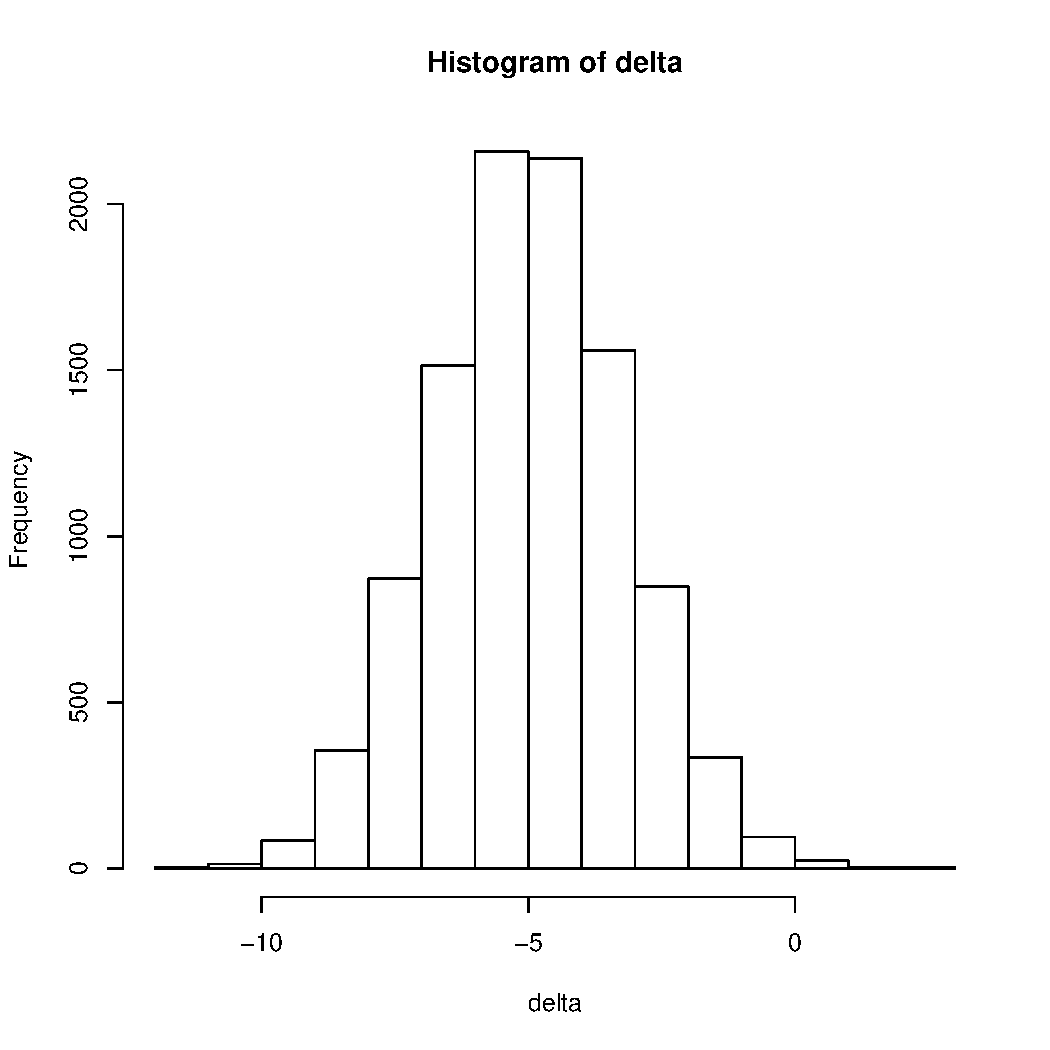
\includegraphics[width=.33\textwidth]{R/mean_diffs_2}};
      \node [below right] at (8,10) {
        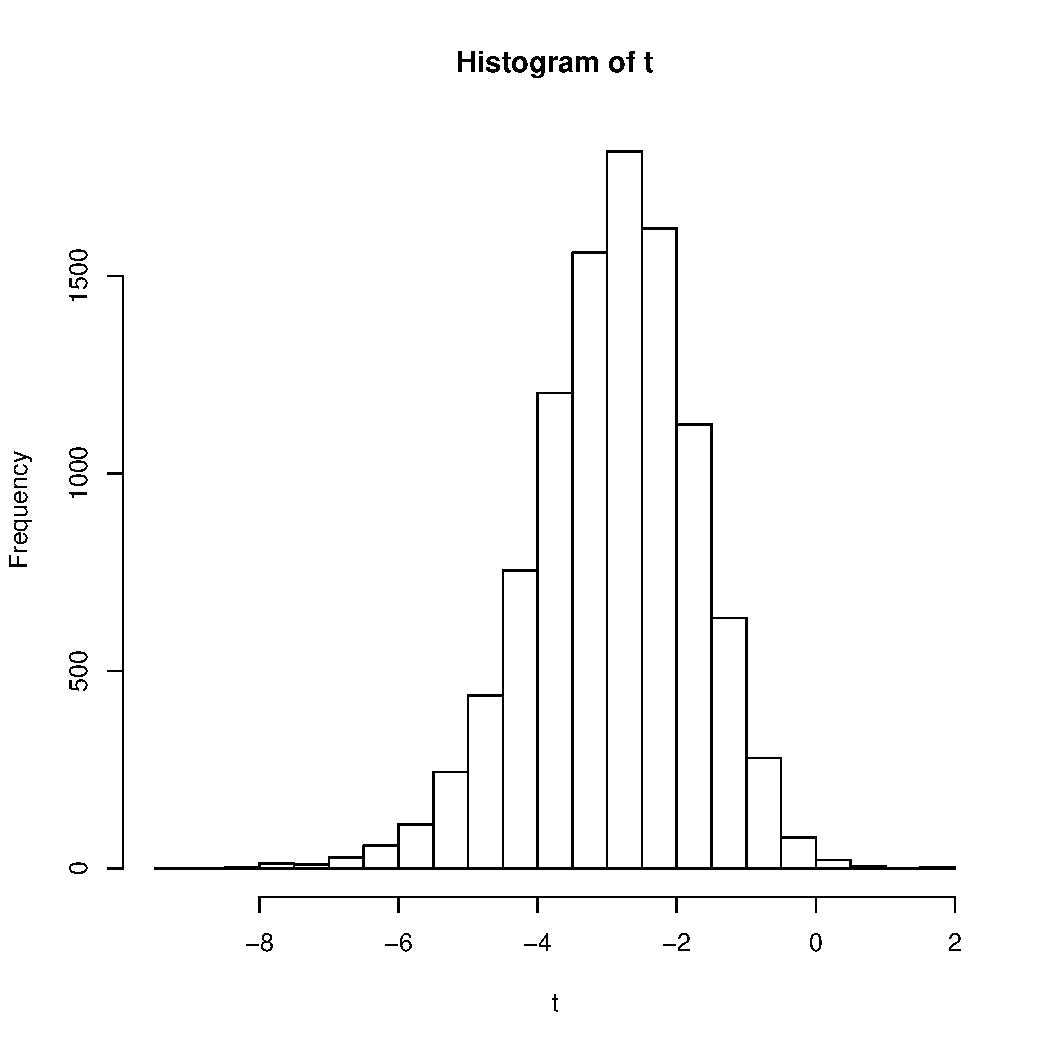
\includegraphics[width=.33\textwidth]{R/t_values_2}};
      \node [below right] at (16,10) { 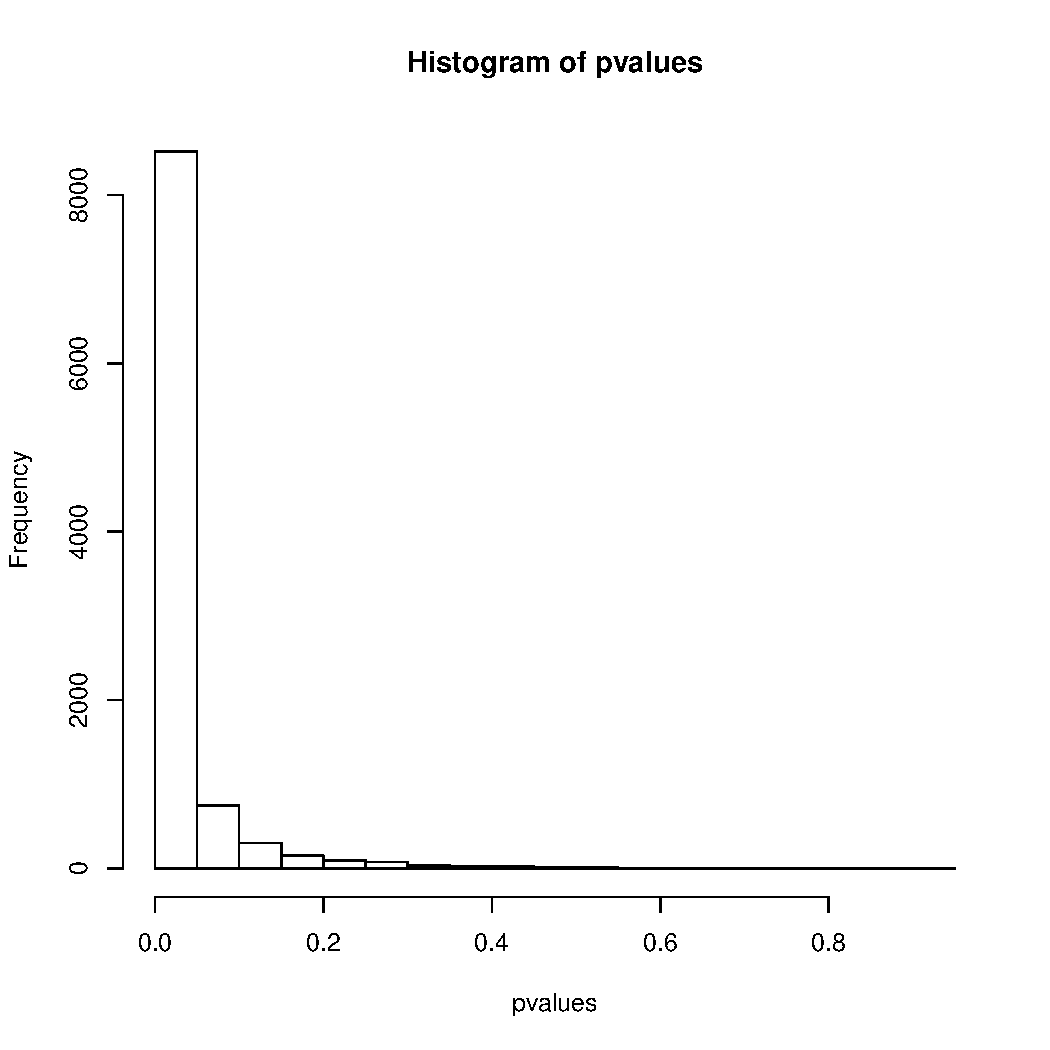
\includegraphics[width=.33\textwidth]{R/p_values_2}};
    \end{tikzpicture}
  \end{figure}
\end{frame}

\begin{frame}[fragile]{with fewer replicates}
  Means are 0 and 5, sd = 4, replicate no=3.
  \begin{figure}[ht]
    \begin{tikzpicture}[scale=0.5]
      \node [below right] at (0,10) {
        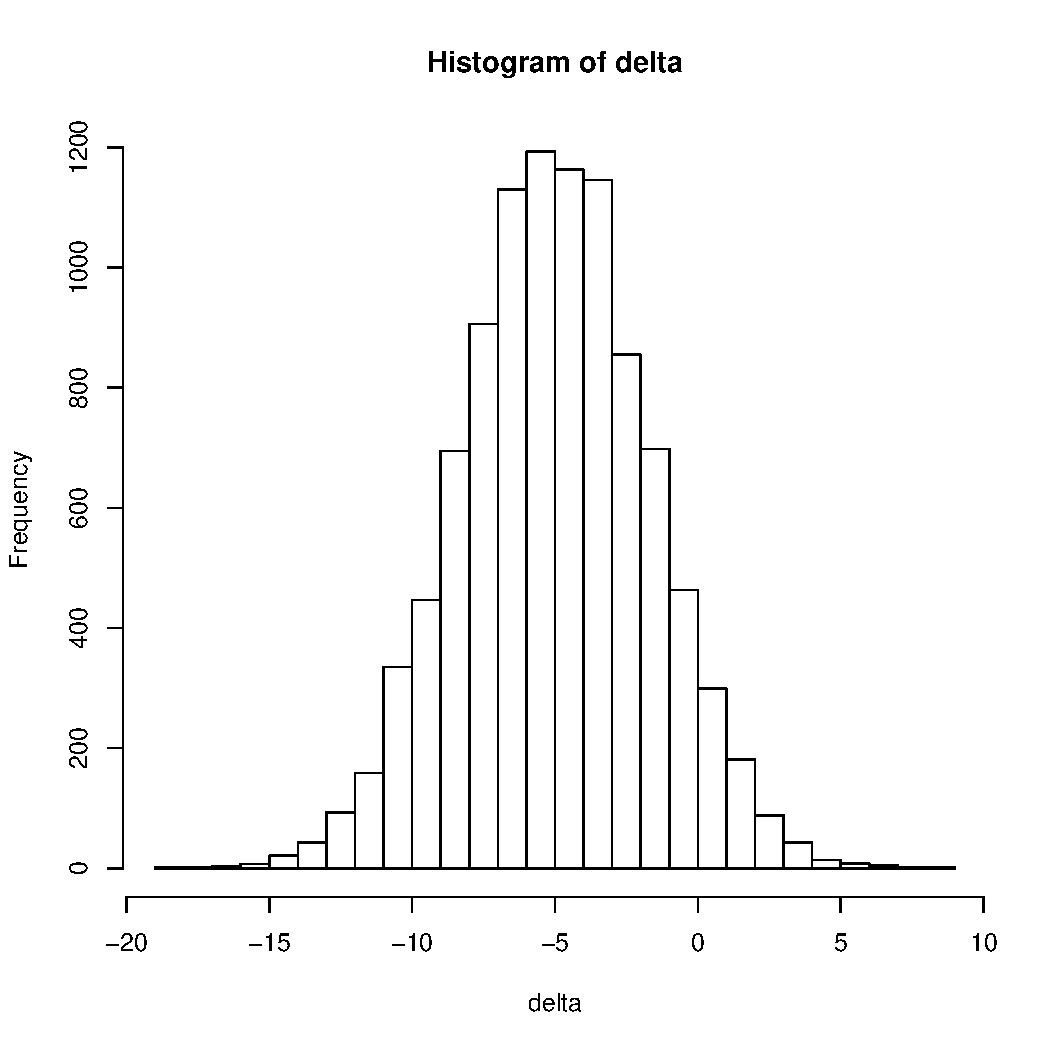
\includegraphics[width=.33\textwidth]{R/mean_diffs_3}};
      \node [below right] at (8,10) {
        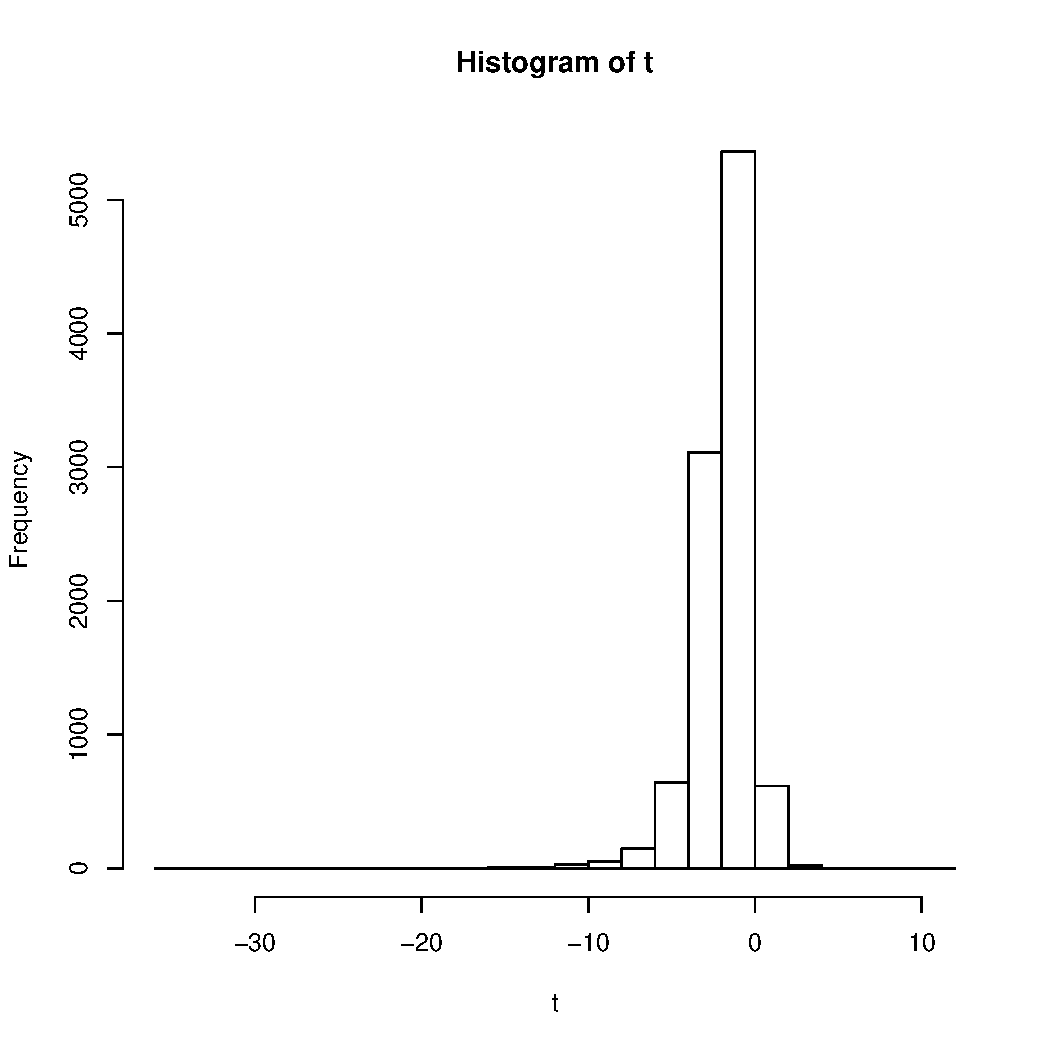
\includegraphics[width=.33\textwidth]{R/t_values_3}};
      \node [below right] at (16,10) { 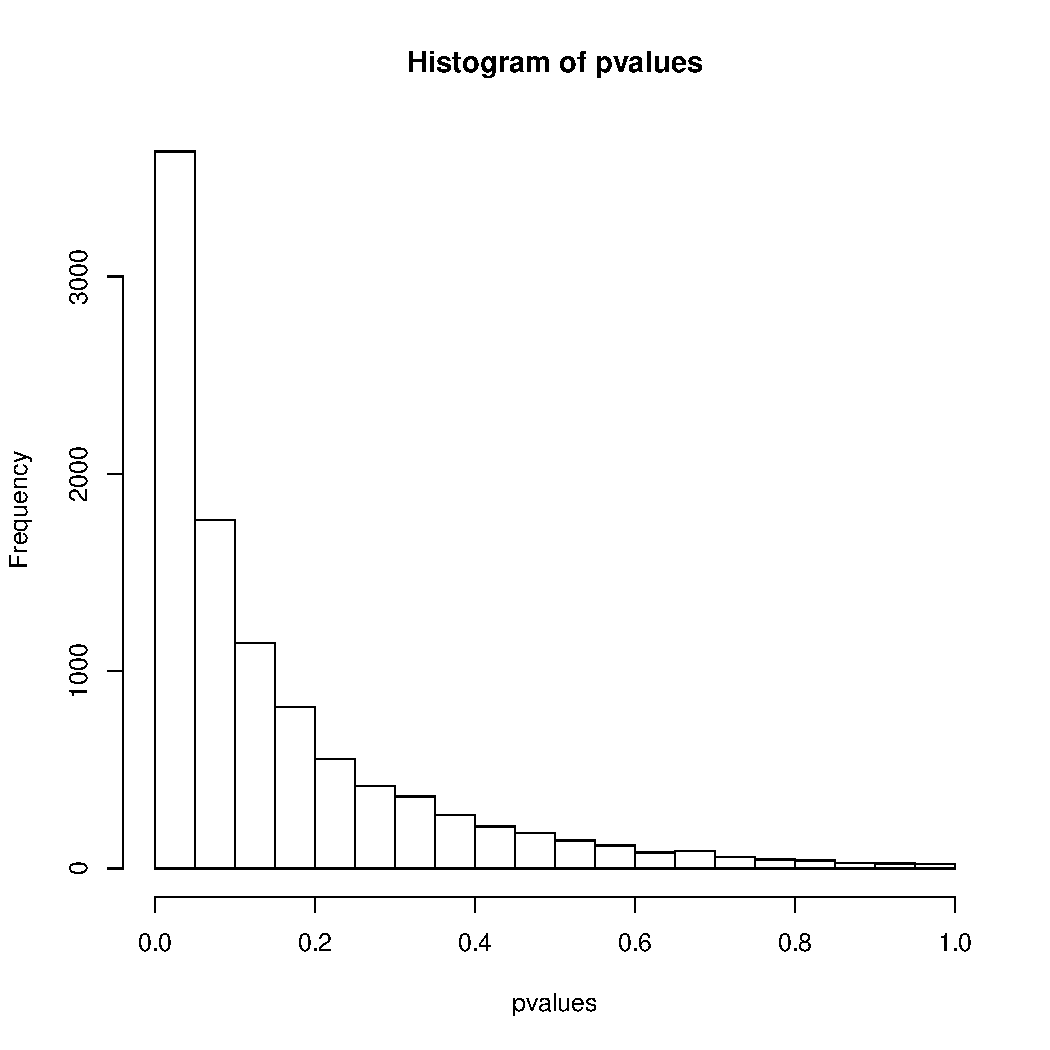
\includegraphics[width=.33\textwidth]{R/p_values_3}};
    \end{tikzpicture}
  \end{figure}
\end{frame}

\begin{frame}{How many replicates?}
  \begin{figure}[ht]
    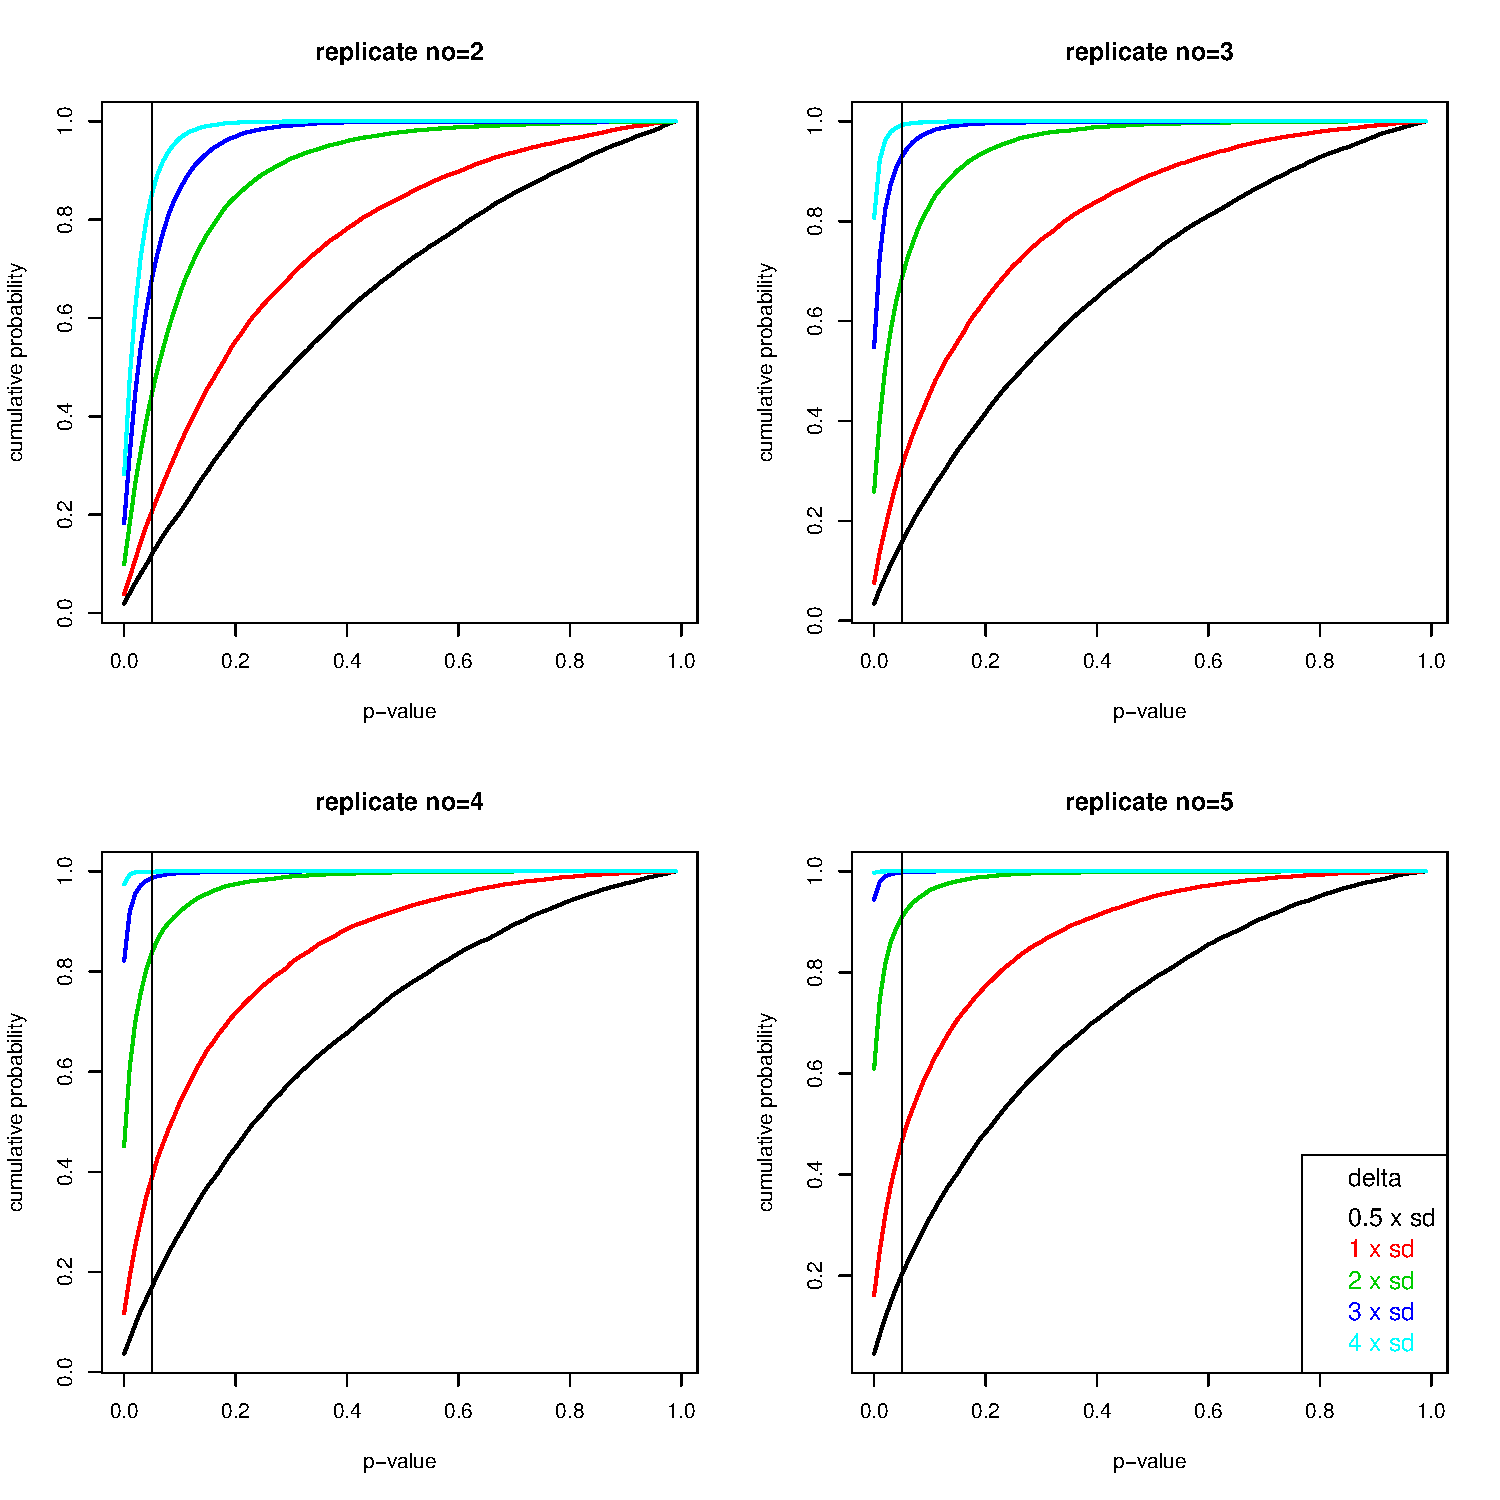
\includegraphics[width=0.75\textwidth]{R/replicate_numbers}
  \end{figure}
\end{frame}
  

\begin{frame}{Not just t-tests}
  \begin{itemize}
  \item The availability of cheap computational power means that it
    is easy to create new statistical tests by simulating the
    experimental data as data sampled from appropriate distributions.
  \item In general this comes under the heading of Monte Carlo simulations
    and is useful for complex systems which are difficult to calculate
    directly.
  \item Also good as an educational tool to explain how we get probabilities
    in statistics.
  \item Or for biologists who may not be very good at maths...
  \end{itemize}
\end{frame}

\begin{frame}{Exercises with numbers}
  \begin{enumerate}
  \item Create two sets of values (X \& Y) by taking the means of random
    variables as above.
  \item Look at how the means of these values differ
  \item Look at the standard deviations
  \item Investigate how this is affected by difference choices of k, minV,
    maxV and n.
  \item Use the built-in R \texttt{rnorm} function to obtain samples of
    standard deviations by specifying the standard deviation and mean values
  \item Keep changing things until you understand everything...
  \end{enumerate}
\end{frame}


\end{document}

